\section{Gasphasenabscheidungen}

Gasphasenabscheidungen sind eine Klasse von Verfahren, bei denen dünne Schichten durch physikalische oder chemische Prozesse aus der Gasphase auf eine Oberfläche aufgetragen werden.
Sie teilen sich in \textbf{Physikalische Gasphasenabscheidung} (PVD, Physical Vapor Deposition), \textbf{Chemische Gasphasenabscheidung} (CVD, Chemical Vapor Deposition) und \textbf{Atomlagenabscheidung} (ALD, Atomic Layer Deposition) auf, die im folgenden betrachtet werden.

Ihnen ist allgemein, dass einzelne Atome oder Moleküle auf der Oberfläche aufkommen, dort physikalisch oder chemisch adsorbiert werden und eventuelle Nebenprodukte aus dem Reaktor gespült werden, wodurch mit vorhersehbarer Rate eine dünne Schicht des Zielmateriales aufwächst.
Tabellen \ref{tab:deposition-comparison} und \ref{tab:deposition-materials} stellen jeweils Charakteristiken und mögliche Materialien für die drei Prozesse dar.

\begin{figure}
  \centering
  \def\svgwidth{\textwidth}
  \input{img/reactors.pdf_tex}
  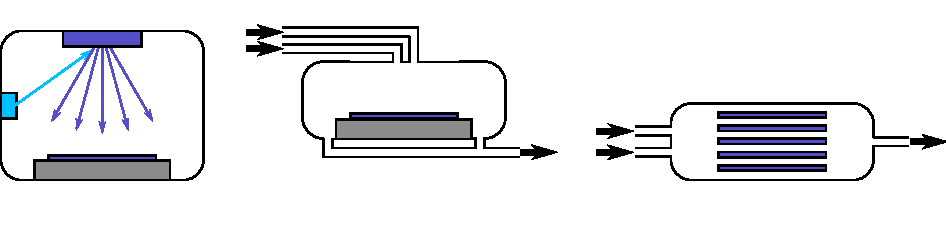
\includegraphics[]{reactors}
  \caption[Abscheidungskammern und -reaktoren]{Abscheidungskammern und -reaktoren}
  \label{fig:reactors}
\end{figure}

\begin{table}
  \centering
  \begin{tabularx}{\textwidth}{|X|ccc|}
    \hline
    Prozesscharakteristiken & \textbf{PVD} & \textbf{CVD} & \textbf{ALD} \\
    \hline
    reaktiv &  & \cmark & \cmark \\
    kontinuierlich & \cmark & \cmark & zyklisch \\
    Gas-Edukte & Atome, Moleküle & Precursor-Moleküle & Precursor-Moleküle \\
    \# Edukte & 1 & 1+ & 2+ \\
    Nebenprodukte & & \cmark & \cmark \\
    Wachstumsrate & $\sim t$ & $\sim t$ & $\sim n_\text{cyc.}$ \\
    \hline
  \end{tabularx}
  \caption[Prozesscharakteristiken der Abscheidungsarten]{Vergleich der Abscheidungsarten}
  \label{tab:deposition-comparison}
\end{table}

\begin{table}
  \centering
  \begin{tabularx}{\textwidth}{XXXXXXXXX}
    & \angled{Metalle} & \angled{Legierungen} & \angled{Metalloxide} & \angled{Nitride} & \angled{Chloride} & \angled{Silizium}  & \angled{Siliziumoxid} & \angled{Diamant} \\
    \hline
    \textbf{PVD} &\cmark&\cmark&&&&\cmark&&?\\
    \textbf{CVD} &\cmark&?&\cmark&\cmark&\cmark&\cmark&?&?\\
    \textbf{ALD} &\cmark&?&\cmark&\cmark&\cmark&\cmark&\cmark&\cmark\\
  \end{tabularx}
  \caption[Mögliche Produkte der Abscheidungsarten]{Mögliche Produkte der Abscheidungsarten. Weitergehende Informationen finden sich in der Literatur für PVD\cite{asd}, CVD\cite{asd} und ALD\cite{puurunen_surface_2005}.}
  \todo[inline]{Referenzen für abgeschiedene Systeme}
  \label{tab:deposition-materials}
\end{table}

\subsection{Physikalische Gasphasenabscheidung}

PVD ist kontinuierlich und nicht reaktiv, arbeitet also mit Atomen oder Molekülen, die physikalisch auf der Oberfläche adsorbieren.
Beispielsweise werden beim Sputtering durch energiereiche Partikel (Argon-Plasma) einzelne Atome aus dem sogenannten Target geschlagen, die dann auf dem Substrat eine homogene, dünne Schicht bilden.
Durch die Nutzung mehrerer Targets (Cosputtering) oder mehrerer Atomsorten in einem Target lassen sich auch Legierungen und andere mehrelementige Materialien abscheiden.
\todo{Referenzen für alles}

\subsection{Chemische Gasphasenabscheidung}

CVD wächst durch chemische Adsorption eines oder mehrerer Precursor-Moleküles eine dünne Schicht auf dem Substrat auf.
Dazu werden die Precursorgase zeitgleich in den Reaktor geleitet, wo sie über die Substratoberfläche strömen und Reaktionen ermöglichen.
Die dabei entstehenden Nebenprodukte werden mit dem Gasstrom aus dem Reaktor geführt, um die aufwachsende Schicht nicht zu verunreinigen.
\todo{zu abrupter Übergang}

Passende Precursor-Kombinationen zu finden, gestaltet sich oft schwierig, da sie idealerweise erst auf der Oberfläche und nicht in der Gasphase reagieren und dabei inerte Nebenprodukte erzeugen sollen.
Weitere Kriterien wie Prozesstemperaturen, Energiebarrieren und komplizierte Reaktionspfade erschweren die Suche zusätzlich.
Im Gegensatz zu PVD kann CVD dafür auf allen Substraten, über deren Oberfläche ein kontinuierlicher Gasfluss möglich ist, eine dünne Schicht abscheiden.
Dies beinhaltet Stufen, Rillen und anderweitig strukturierte Substrate ebenso wie Poren durch das Substrat.

\missingfigure{Beispiel Precursor-Moleküle}

\subsection{Atomlagenabscheidung}

\begin{figure}
  \centering
  \def\svgwidth{\textwidth}
  \input{img/ald-schema.pdf_tex}
  \caption[ALD-Schema]{ALD-Schema: dsa ald}
  \label{fig:ald-schema}
\end{figure}

Als Variation von CVD entstand ALD \todo{Referenz} mit dem Ziel, dünne Schichten kontrolliert in einzelnen Atomlagen abzuscheiden.
Dazu werden zwei Precursorgase in wechselweisen Schritten in den Reaktor geleitet, zwischen denen Spülschritte mit inertem Gas verbleibende Moleküle und Nebenprodukte aus dem Reaktor spülen (Abbildung \ref{fig:ald-schema}).
So werden einerseits Gasphasenreaktionen vermieden, andererseits sorgt die Sättigung \todo{Grafik zur Sättigung} der Oberfläche mit Precursorliganden in jedem Precursorschritt für zyklen-begrenztes Schichtwachstum.
Anders als der Name vermuten lässt, werden aber normalerweise keine kompletten Monolagen in einem Zyklus aufgebracht.
Üblicherweise erreichen ALD-Prozesse bis zu 35\% \todo{referenz} einer Monolage, bedingt durch sterische Hinderung (Abbildung \ref{fig:steric}).
Die Wachstumsrate wird somit von dem Growth-per-Cycle-Wert (GPC) abgelöst, der angibt, wie stark eine Schicht im Schnitt pro Zyklus wächst.

Große Gruppen von Precursorliganden verhindern durch sterische Hinderung einen hohen GPC-Wert, weshalb kompakte Precursor bevorzugt untersucht werden. \todo{Referenz?}
Die Suche nach möglichen Precursorpaaren und Prozessparametern unterliegt ansonsten gleichen Anforderungen wie bei CVD.

Eine ausführlichere Übersicht zu Atomlagenabscheidung und mögliche Precursorpaare findet sich in Referenz \cite{puurunen_surface_2005}.

\begin{figure}
  \centering
  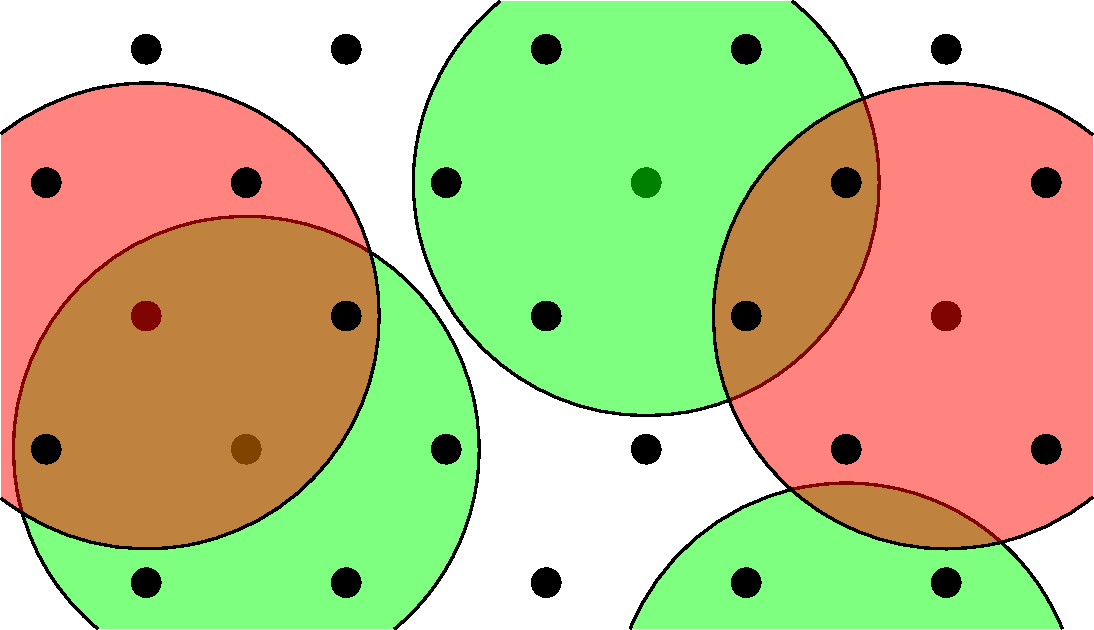
\includegraphics[width=0.5\textwidth]{sterichindrance}
  \caption[Sterische Hinderung]{Sterische Hinderung auf einem Gitter:
    Angelagerte Precursor-Liganden verhindern Reaktionen auf benachbarten Gitterpunkten.
    Überlagerungsfreie Positionen in größerem Abstand akzeptieren weiterhin Precursor-Reaktionen.
  }
  \label{fig:steric}
\end{figure}

\subsection{Simulation von Gasphasenabscheidungen}

\begin{table}
  \centering
  \begin{tabularx}{\textwidth}{XXXX}
    \hline
    Methode & Anwendungsfeld & Größenordnung & Grundlagen \\
    \hline
    Finite Elemente Methode (FEM) & Gasfluss und Verbrauch in Reaktoren & makroskopisch & Navier-Stokes-Gl., Reaktionskinetik \\
    Kinetic Monte Carlo (KMC) & Wachstums\-simulationen & mikroskopisch & Reaktionsraten, Gitternäherungen \\
    Molekular\-dynamik (MD) & Material\-unter\-suchungen & < 1.000.000 Atome & klassische Interaktionspotentiale \\
    Dichte\-funktional\-theorie (DFT) & Reaktionspfade & < 1.000 Atome & Elektronendichten \\
    \hline
  \end{tabularx}
  \caption[Ausgewählte Methoden zur Simulation von Gasphasenabscheidungen]{Ausgewählte Methoden zur Simulation von Gasphasenabscheidungen}
  \label{tab:deposition-simulations}
  \todo[inline]{Referenzen!}
\end{table}

Tabelle \ref{tab:deposition-simulations} stellt ausgewählte Simulationsmethoden für Gasphasenabscheidungen vor, die in der Praxis Anwendung finden.
Besonders auf atomarer Ebene sind viele Prozesse nicht vollends verstanden.
So ist der genaue Reaktionspfad für Precursorpaare oft nicht bekannt, obwohl sie seit Jahrzehnten erfolgreich eingesetzt werden.
Durch Simulationen will man diese Prozesse verstehen helfen und somit genauere Kontrolle über die abgeschiedenen Schichten erlangen.

Dichtefunktionaltheorie und Molekulardynamik stechen hier aufgrund ihrer atomaren Arbeitsweise besonders hervor.
DFT-Untersuchungen beschränken sich hier auf die Reaktionspfade von Molekülen, wo hingegen Molekulardynamik das fertige Material zu simulieren versucht.
In den letzten Jahren sind hingegen auch reaktive Formulierungen für Molekulardynamik aufgekommen\todo{Referenz}, die einen zentralen Bestandteil dieser Arbeit bilden.
